\documentclass[tikz,border=4pt]{standalone}
\usepackage{pgfplots}
\pgfplotsset{compat=1.18}
\usetikzlibrary{patterns}

\definecolor{singleblue}{RGB}{67,113,159}
\definecolor{hiedorange}{RGB}{244,126,28}
\definecolor{textgray}{RGB}{54,60,66}

\begin{document}
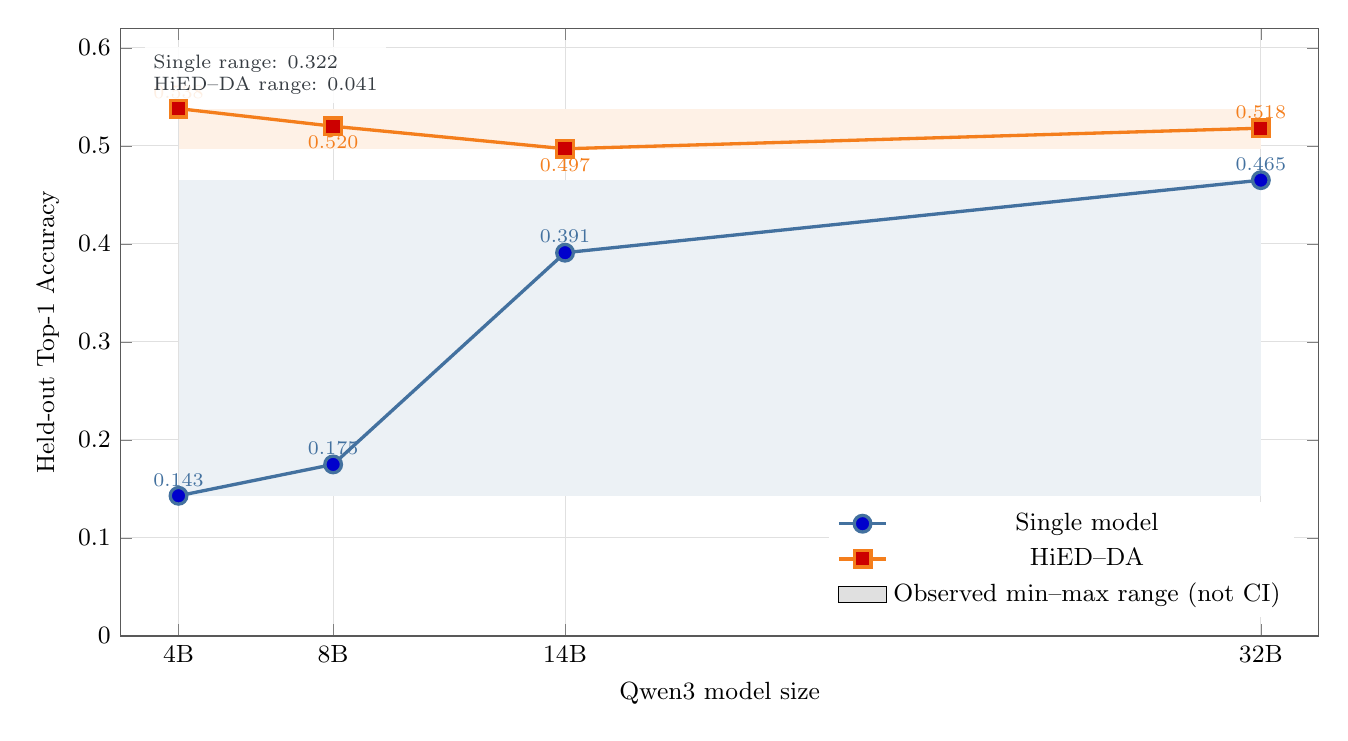
\begin{tikzpicture}
\begin{axis}[
  width=16.8cm,
  height=9.3cm,
  xmin=2.5, xmax=33.5,
  ymin=0, ymax=0.62,
  xtick={4,8,14,32},
  xticklabels={4B,8B,14B,32B},
  xlabel={Qwen3 model size},
  ylabel={Held-out Top-1 Accuracy},
  tick label style={font=\small},
  label style={font=\small},
  grid=major,
  major grid style={draw=black!12},
  axis line style={draw=black!65},
  legend style={
    font=\small,
    draw=none,
    fill=white,
    at={(0.98,0.03)},
    anchor=south east,
    row sep=1pt
  },
  clip=false
]

% Observed min--max bands across the four evaluated sizes. These are not confidence intervals.
\path[fill=singleblue!10, draw=none] (axis cs:4,0.143) rectangle (axis cs:32,0.465);
\path[fill=hiedorange!11, draw=none] (axis cs:4,0.497) rectangle (axis cs:32,0.538);

\addplot+[singleblue, very thick, mark=*, mark size=3pt] coordinates {
  (4,0.143) (8,0.175) (14,0.391) (32,0.465)
};
\addlegendentry{Single model}

\addplot+[hiedorange, very thick, mark=square*, mark size=3pt] coordinates {
  (4,0.538) (8,0.520) (14,0.497) (32,0.518)
};
\addlegendentry{HiED--DA}

\addlegendimage{area legend, fill=black!12, draw=none}
\addlegendentry{Observed min--max range (not CI)}

\node[font=\scriptsize, text=singleblue, anchor=south] at (axis cs:4,0.143) {0.143};
\node[font=\scriptsize, text=singleblue, anchor=south] at (axis cs:8,0.175) {0.175};
\node[font=\scriptsize, text=singleblue, anchor=south] at (axis cs:14,0.391) {0.391};
\node[font=\scriptsize, text=singleblue, anchor=south] at (axis cs:32,0.465) {0.465};

\node[font=\scriptsize, text=hiedorange, anchor=south] at (axis cs:4,0.538) {0.538};
\node[font=\scriptsize, text=hiedorange, anchor=north] at (axis cs:8,0.520) {0.520};
\node[font=\scriptsize, text=hiedorange, anchor=north] at (axis cs:14,0.497) {0.497};
\node[font=\scriptsize, text=hiedorange, anchor=south] at (axis cs:32,0.518) {0.518};

\node[font=\scriptsize, text=textgray, anchor=north west, align=left, fill=white, fill opacity=0.88, text opacity=1, inner sep=3pt]
  at (rel axis cs:0.02,0.97)
  {Single range: 0.322\\HiED--DA range: 0.041};

\end{axis}
\end{tikzpicture}
\end{document}
